% IEEE Access-style manuscript.
% NOTE: the official ieeeaccess.cls was not available when this was prepared, so the local
% approximation ieeeaccessapprox.cls is used. For submission, move the body into the official
% IEEE Access template (https://ieeeaccess.ieee.org/) and use \documentclass{ieeeaccess}.
\documentclass{ieeeaccessapprox}
\usepackage{amsmath,amssymb}
\usepackage{graphicx}
\usepackage{booktabs}
\usepackage{multirow}
\usepackage{url}
\usepackage{enumitem}
\usepackage{cite}
\usepackage{dblfloatfix}
\usepackage[hidelinks,pdfusetitle]{hyperref}
\newcommand{\nParams}{1{,}055{,}081}
\newcommand{\nMACsG}{2.53}
\newcommand{\nSpatial}{883{,}472}
\newcommand{\nTemporal}{37{,}968}
\newcommand{\nFusion}{132{,}480}
\newcommand{\nHeads}{1{,}161}
\newcommand{\pSpatial}{83.7}
\newcommand{\pTemporal}{3.6}
\newcommand{\pFusion}{12.6}
\newcommand{\pBlockOne}{54}
\newcommand{\pBlocksOneTwo}{82}
\newcommand{\nWithin}{149}
\newcommand{\nTrials}{150}
\newcommand{\nMainsDb}{22}
\newcommand{\ampBefore}{0.152}
\newcommand{\ampAfter}{0.0125}
\newcommand{\noiseRef}{0.0212}
\newcommand{\notchLo}{49.18}
\newcommand{\notchHi}{50.83}
\newcommand{\notchW}{1.65}
\newcommand{\notchDb}{97}
\newcommand{\oneHzDb}{5.8}
\newcommand{\gdTen}{6.1}
\newcommand{\gdTwenty}{3.1}
\newcommand{\gdThirty}{2.8}
\newcommand{\covTotal}{95.1}
\newcommand{\nStmts}{548}
\newcommand{\nHit}{521}
\newcommand{\covTrain}{75.3}
\newcommand{\nFullMods}{8}
\newcommand{\nMods}{12}
\newcommand{\atrophyROI}{40}
\newcommand{\lesionROI}{180}
\newcommand{\retLesion}{99.7}
\newcommand{\retAtrophy}{0}

\newcommand{\todo}[1]{\colorbox{yellow}{[#1]}}
\newcommand{\cafn}{CAFN}
\def\UrlBreaks{\do\/\do\-\do\_\do\.\do\=}
\setlist[itemize]{leftmargin=1.2em,itemsep=1pt,topsep=2pt,parsep=0pt}
\setlist[enumerate]{leftmargin=1.5em,itemsep=1pt,topsep=2pt,parsep=0pt}

\history{Date of publication xxxx 00, 0000, date of current version xxxx 00, 0000.}
\doi{10.1109/ACCESS.2026.DOI}

\title{A Cross-Attention Deep Learning Framework for Multimodal Neuroimaging Fusion in Vision Defect Detection and Classification: Design and Verification on Synthetic Data}

\author{\uppercase{Mishthi Jain}\authorrefmark{1}}
\address[1]{School of Computer Science and Engineering, Vellore Institute of Technology, Chennai, India (e-mail: \todo{author e-mail})}
\tfootnote{This work was carried out as a BCSE497J project at the School of Computer Science and Engineering, Vellore Institute of Technology, Chennai. \todo{funding statement, if any}}
\markboth{M. Jain: Cross-Attention Fusion of 3D MRI and Visual Evoked Potentials}{M. Jain: Cross-Attention Fusion of 3D MRI and Visual Evoked Potentials}
\corresp{Corresponding author: Mishthi Jain (e-mail: \todo{author e-mail}).}

\begin{document}
\maketitle

\begin{abstract}
Disorders of the visual pathway, such as glaucoma, optic neuritis and cortical visual impairment, alter both the structure of the pathway, seen on structural magnetic resonance imaging (MRI), and the timing of its electrical response, recorded as the visual evoked potential (VEP). Most computational tools use only one of the two. This paper presents the Cross-Attention Fusion Network (CAFN), an open-source research prototype that classifies a paired 3D MRI volume and 1D VEP waveform as Healthy Control, Glaucoma, or Optic Neuritis/Cortical Visual Impairment. A 3D residual network and a 1D convolutional network map the inputs to 64 spatial and 16 temporal tokens; multi-head cross-attention, with spatial tokens as queries and temporal tokens as keys and values, fuses them, and two auxiliary unimodal heads regularise training. Zero-phase filtering preserves the P100 latency, and 3D Grad-CAM and an attention heatmap provide inspection aids. Because no public dataset offers the required diagnosis labels, the system is developed and verified on class-conditioned synthetic data. On \nTrials{} synthetic recordings the conditioning chain recovered the P100 latency within one sample (4 ms) in \nWithin{} cases and attenuated injected 50 Hz interference by \nMainsDb{} dB on average. The model has 1.06 million parameters and about \nMACsG{} billion multiply--accumulate operations per sample, and an 86-test suite covers \covTotal\% of statements. No diagnostic accuracy is claimed; the contribution is a tested, configuration-driven foundation for evaluation on a labelled clinical cohort.
\end{abstract}

\begin{keywords}
Cross-attention, deep learning, explainability, glaucoma, magnetic resonance imaging, multimodal fusion, optic neuritis, visual evoked potentials.
\end{keywords}

\titlepgskip=-15pt

\section{Introduction}
\PARstart{V}{ision} depends on an uninterrupted chain of structures: the retina, the optic nerve, the optic chiasm, the lateral geniculate nucleus, the optic radiations and the visual cortex. A lesion anywhere along the chain can degrade sight, and the clinical picture depends on where the damage lies and on whether it disturbs the anatomy, the conduction of the electrical signal, or both. Glaucoma, a progressive optic neuropathy, had an estimated global prevalence of 3.54\% among people aged 40 to 80 years, or about 64.3 million people in 2013 \cite{tham2014}, and its degeneration is not confined to the eye but extends to the intracranial optic nerve, the lateral geniculate nucleus and the visual cortex \cite{gupta2006}. Optic neuritis, an inflammatory disorder of the optic nerve, is characterised electrophysiologically by a delayed P100 peak of the VEP \cite{halliday1972}. Cortical (or cerebral) visual impairment (CVI) arises from damage to the brain's visual pathways, and the terminology used for it varies widely \cite{sakki2018}.

Two investigations are routinely used to examine this pathway, and they answer different questions. Structural MRI gives a three-dimensional picture of anatomy, so that atrophy and focal lesions can be localised, but it carries no timing information. The VEP is a one-dimensional recording of the cortical response to a visual stimulus whose latency and amplitude, in particular those of the P100 component, reflect the integrity and conduction speed of the pathway \cite{odom2016}, but it carries no spatial localisation. Combining complementary modalities has long been proposed as a way to reveal relationships that no single modality shows \cite{calhoun2016}.

Learning such a combination faces three obstacles. First, most computational pipelines analyse either imaging or electrophysiology, not both (\emph{unimodal isolation}). Second, a volume and a waveform differ in dimensionality, sampling and noise, and simple fusion by concatenation gives every feature the same standing (\emph{cross-modal heterogeneity}). Third, a black-box classifier is difficult to trust clinically (\emph{limited interpretability}). A further, practical obstacle is the absence of public datasets with paired MRI, VEP and diagnosis labels.

This paper describes and verifies the Cross-Attention Fusion Network (CAFN), a research prototype that addresses the first three obstacles within an architecture that can be exercised end to end before a labelled cohort exists. Its contributions are:
\begin{enumerate}
\item an architecture in which spatial tokens from a 3D residual CNN act as \emph{queries} that select relevant temporal tokens from a 1D CNN, trained with a fused head and two auxiliary unimodal heads;
\item a zero-phase VEP conditioning chain designed to preserve P100 latency, with a quantitative analysis of its frequency response, mains attenuation and latency recovery;
\item a class-conditioned synthetic data generator that exposes the same file interface as real data, so that the complete path from NIfTI and CSV files to an optimiser step and to explanation maps can be tested;
\item an analytic account of model size and cost and an automated test suite (86 tests, \covTotal\% statement coverage), together with an explicit statement of what this evidence does \emph{not} show.
\end{enumerate}
The source code is available at \url{https://github.com/Mishthijainn/NeuroImaging}. The rest of the paper reviews related work (Section~\ref{sec:related}), describes the framework (Section~\ref{sec:method}) and the evaluation protocol (Section~\ref{sec:setup}), reports the results (Section~\ref{sec:results}), discusses their meaning and limits (Section~\ref{sec:discussion}), and concludes (Section~\ref{sec:conclusion}).

\section{Related Work}\label{sec:related}
\subsection{Deep learning for volumetric neuroimaging}
Three-dimensional CNNs are the standard tool for learning directly from volumetric scans: efficient multi-scale 3D CNNs were developed for brain-lesion segmentation \cite{kamnitsas2017}, and the 3D U-Net showed dense volumetric segmentation from sparse annotation \cite{cicek2016}. Residual connections \cite{he2016} are routinely carried over to 3D, as in the spatial encoder used here. Volumetric pipelines also depend on preprocessing: brain extraction is a prerequisite for many analyses, and dedicated tools exist, such as HD-BET \cite{isensee2019} and SynthStrip \cite{hoopes2022}; MONAI offers open-source transforms for resampling and cropping \cite{cardoso2022}. The present work uses MONAI transforms but replaces skull-stripping with an explicitly labelled placeholder (Section~\ref{sec:mri}).

\subsection{Evoked-potential conditioning and 1D CNNs}
Evoked potentials are conventionally conditioned to remove baseline drift, muscle noise and mains interference before analysis. A Butterworth filter has a maximally flat pass-band \cite{butterworth1930}, and a narrow IIR notch removes the mains frequency. Applying a filter forward and then backward over the record cancels its phase response \cite{gustafsson1996,oppenheim2010}, which matters because clinical interpretation of the VEP rests on latency \cite{odom2016}. One-dimensional CNNs then learn local temporal patterns with learned filters.

\subsection{Multimodal fusion and cross-attention}
Surveys of multimodal learning distinguish early, intermediate and late fusion according to where modalities are combined \cite{baltrusaitis2019,ramachandram2017}. Early fusion is ill-suited to a volume and a waveform, which share no natural input space; late fusion forgoes interaction before the decision; intermediate fusion by concatenation weights all features equally. Scaled dot-product attention lets queries select among keys and values \cite{vaswani2017}, vision transformers treat images as sequences of patch tokens \cite{dosovitskiy2021}, and cross-modal attention has been used to relate modalities that are not time-aligned \cite{tsai2019,lu2019}. CAFN applies this idea to MRI and VEP.

\subsection{Explainability}
Grad-CAM uses class-score gradients with respect to convolutional activations to produce a coarse localisation map \cite{selvaraju2017}. Attention weights are not automatically faithful explanations \cite{jain2019}, although whether they can serve as explanations depends on how the question is posed \cite{wiegreffe2019}, and saliency maps can be insensitive to a model's parameters \cite{adebayo2018}. The explainability outputs here are therefore treated as inspection aids.

\subsection{Public data and the labelling gap}
Public resources exist for structural and functional neuroimaging and electrophysiology, including the Human Connectome Project and its 7~T retinotopy data \cite{vanessen2013,benson2018}, OASIS-3 \cite{lamontagne2019}, the MNE-Python sample data \cite{gramfort2013} and PhysioNet \cite{goldberger2000}. They support preprocessing development and retinotopic mapping, but none provides the Healthy/Glaucoma/Optic-Neuritis-CVI diagnosis labels with paired MRI and VEP that this task requires. A labelled, paired clinical cohort is therefore still needed, which is why the synthetic generator of Section~\ref{sec:synth} is used.

\section{The CAFN Framework}\label{sec:method}
\subsection{Overview}
CAFN takes a paired sample consisting of a 3D MRI volume and a 1D VEP record and predicts one of three classes (Healthy Control, Glaucoma, Optic Neuritis/CVI). Figure~\ref{fig:pipeline} shows the data flow and Table~\ref{tab:shapes} the tensor shapes at the default configuration, which is held in a single configuration module so that preprocessing, both encoders, the fusion module and the training loop cannot disagree on shapes.

\begin{figure*}[!t]
\centering
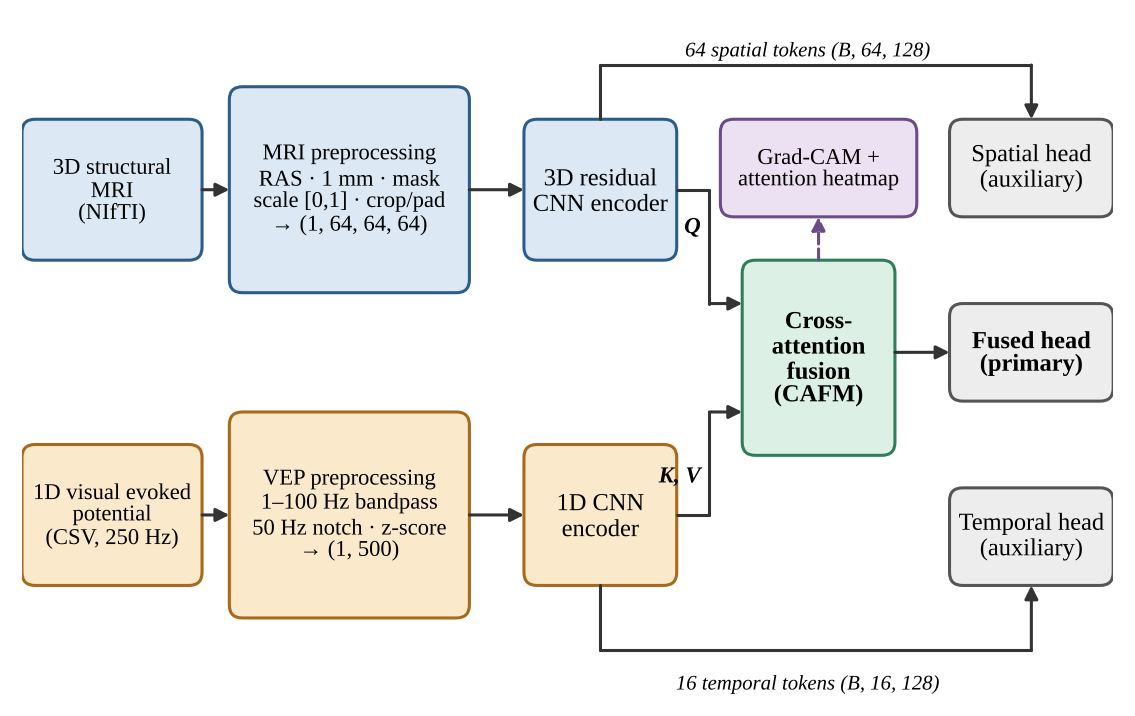
\includegraphics[width=0.66\textwidth]{figs/fig_pipeline.png}
\caption{End-to-end data flow of CAFN. Spatial tokens act as queries ($Q$) and temporal tokens as keys and values ($K,V$) of the cross-attention fusion module (CAFM). The dashed arrow indicates the explainability outputs.}
\label{fig:pipeline}
\end{figure*}

\begin{table}[!t]
\caption{Tensor shapes at the default configuration ($B$: batch size).}
\label{tab:shapes}
\centering\footnotesize
\begin{tabular}{@{}lll@{}}
\toprule
Stage & MRI stream & VEP stream\\
\midrule
After preprocessing & $(1,64,64,64)$ & $(1,500)$\\
Encoder output (tokens) & $(B,64,128)$ & $(B,16,128)$\\
Attention weights & \multicolumn{2}{c}{$(B,4,64,16)$}\\
Fused tokens & \multicolumn{2}{c}{$(B,64,128)$}\\
Logits (3 heads) & \multicolumn{2}{c}{$(B,3)$ each}\\
\bottomrule
\end{tabular}
\end{table}

\subsection{MRI preprocessing}\label{sec:mri}
The MRI stream loads a NIfTI file with NiBabel, reorients it to the closest canonical (RAS) frame, resamples it to 1~mm isotropic spacing with MONAI's trilinear \texttt{Resize}, applies a foreground mask, scales intensities to $[0,1]$ and pads or crops to $64\times64\times64$. The mask zeroes all voxels below the 60th percentile of the strictly positive voxels. This is a lightweight stand-in for skull-stripping, isolated in one function so that a validated tool can replace it; it is \emph{not} clinical-grade brain extraction.

\subsection{VEP conditioning}\label{sec:vep}
The VEP stream validates the record (one-dimensional, finite, non-empty), applies a fourth-order Butterworth band-pass (1--100~Hz) and a 50~Hz IIR notch ($Q=30$), resamples linearly to 500 samples (2~s at 250~Hz) and z-scores. Both filters are applied forward and backward (\texttt{sosfiltfilt} and \texttt{filtfilt}). If $H(j\omega)$ is the single-pass response, the effective response is
\begin{equation}
H_{\mathrm{zp}}(\omega)=\lvert H(j\omega)\rvert^{2},\qquad \arg H_{\mathrm{zp}}(\omega)=0,
\label{eq:zp}
\end{equation}
so waveform timing, and hence P100 latency, is not shifted. Normalisation is $\hat{x}_k=(x_k-\mu)/(\sigma+\varepsilon)$ with $\varepsilon=10^{-8}$.

\subsection{Spatial encoder}
A 3D residual CNN maps the preprocessed volume to 64 tokens. A stem (Conv3d $1\!\to\!16$, batch normalisation, ReLU) is followed by three residual blocks ($16\!\to\!32$, $32\!\to\!64$, $64\!\to\!128$ channels, stride 2), each with two $3\!\times\!3\!\times\!3$ convolutions and an identity or $1\!\times\!1\!\times\!1$ shortcut. The final $8\!\times\!8\!\times\!8$ feature map is average-pooled to $4\!\times\!4\!\times\!4$ and flattened to $X_s\in\mathbb{R}^{64\times128}$. The last residual block is the Grad-CAM target layer.

\subsection{Temporal encoder}
A four-stage 1D CNN (Conv1d with kernel sizes 7, 5, 5, 3; channels $1\!\to\!16\!\to\!32\!\to\!64\!\to\!128$; strides 1, 2, 2, 2; batch normalisation and ReLU) reduces the 500-sample record to a 63-sample feature sequence, which is adaptively pooled to 16 tokens, $X_t\in\mathbb{R}^{16\times128}$. The tokens are learned features; each nominally spans 125~ms of the 2~s record, but they are not calibrated time bins.

\subsection{Cross-attention fusion}
Spatial tokens query the temporal tokens (Fig.~\ref{fig:cross}). With $H=4$ heads and $d_h=d_{\mathrm{model}}/H=32$,
\begin{equation}
Q=X_sW_Q,\quad K=X_tW_K,\quad V=X_tW_V,
\end{equation}
\begin{equation}
A_h=\mathrm{softmax}\!\left(\frac{Q_hK_h^{\top}}{\sqrt{d_h}}\right),\qquad O_h=A_hV_h,
\end{equation}
\begin{equation}
Z=\mathrm{LN}\big(X_s+\mathrm{Concat}(O_1,\dots,O_H)W_O\big),\quad F=\mathrm{LN}\big(Z+\mathrm{FFN}(Z)\big),
\label{eq:fuse}
\end{equation}
where LN is layer normalisation and FFN is a two-layer network ($128\!\to\!256\!\to\!128$, ReLU, dropout 0.1). The attention tensor has shape $(B,4,64,16)$, each row sums to one, and it is returned for inspection. The fused tokens $F\in\mathbb{R}^{64\times128}$ keep the spatial layout and are enriched with temporal context.

\begin{figure}[!t]
\centering
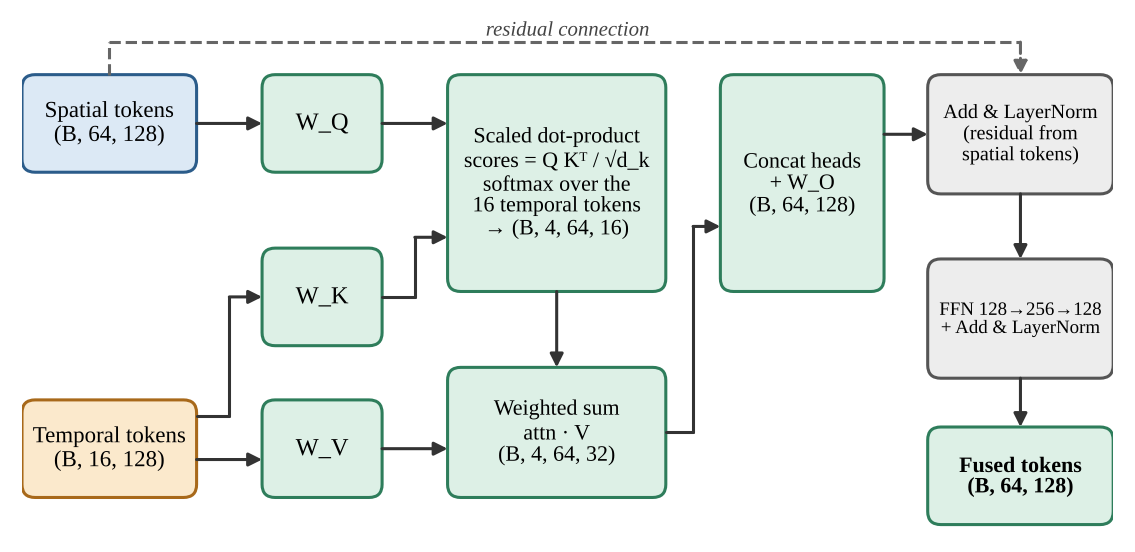
\includegraphics[width=\columnwidth]{figs/fig_cross_attention.png}
\caption{Cross-attention fusion module. The attention tensor has shape $(B,4,64,16)$ and is returned for inspection.}
\label{fig:cross}
\end{figure}

\subsection{Multi-task objective}
Three linear heads ($128\!\to\!3$) read the mean-pooled fused tokens, spatial tokens and temporal tokens. The fused head is the primary classifier; the auxiliary heads give each encoder its own gradient signal and discourage the fused head from ignoring one modality. With cross-entropy losses $L_f$, $L_s$ and $L_t$,
\begin{equation}
L_{\mathrm{total}}=L_f+\lambda\,(L_s+L_t),\qquad\lambda=0.3 .
\end{equation}
Training uses Adam, learning rate $10^{-3}$, weight decay $10^{-4}$, batch size 8, 20 epochs, a 20\% seeded validation split and seed 42.

\subsection{Explainability outputs}
\emph{3D Grad-CAM} registers hooks on the last residual block, back-propagates from the fused logit $y^c$, and forms
\begin{equation}
\alpha_k=\frac{1}{Z}\sum_{i,j,l}\frac{\partial y^c}{\partial A^k_{ijl}},\qquad M=\mathrm{ReLU}\Big(\sum_k\alpha_kA^k\Big),
\end{equation}
which is upsampled trilinearly to the input size and min--max normalised. The \emph{attention heatmap} averages the attention tensor over batch and heads to a $64\times16$ matrix of spatial token versus temporal token. Both are inspection aids, not clinical evidence (Section~\ref{sec:discussion}).

\subsection{Synthetic data generator}\label{sec:synth}
Because labelled paired data are unavailable, a seeded generator writes class-conditioned MRI volumes and VEP records through the same NIfTI/CSV interface as real data. An MRI volume of shape $80\times96\times64$ is drawn from $\mathcal{N}(100,15^2)$; for Glaucoma the intensities in one octant-sized block are multiplied by 0.4 (atrophy proxy), and for Optic Neuritis/CVI those in another block by 1.8 (lesion proxy). A VEP is a sum of three Gaussians modelling the N75--P100--N145 complex,
\begin{equation}
\begin{split}
s(t)={}&A\,e^{-\frac{(t-\tau)^2}{2\sigma_1^2}}-0.5A\,e^{-\frac{(t-\tau+0.025)^2}{2\sigma_2^2}}\\
&-0.4A\,e^{-\frac{(t-\tau-0.045)^2}{2\sigma_3^2}},
\end{split}
\end{equation}
with $\sigma_{1,2,3}=12,10,15$~ms and $(\tau,A)=(100\,\mathrm{ms},6.0)$, $(108\,\mathrm{ms},2.5)$ and $(140\,\mathrm{ms},4.0)$ for Healthy Control, Glaucoma and Optic Neuritis/CVI, plus a 0.3~Hz baseline drift (amplitude 0.3), 50~Hz mains interference (amplitude 0.15) and Gaussian noise (SD 0.3). These are the very artefacts that the conditioning chain is designed to remove.

\section{Experimental Setup}\label{sec:setup}
\subsection{Implementation}
CAFN is implemented in Python with PyTorch \cite{paszke2019}, MONAI \cite{cardoso2022}, NiBabel, SciPy \cite{virtanen2020} and NumPy \cite{harris2020}; figures use Matplotlib \cite{hunter2007}. All random processes are seeded.

\subsection{Evaluation protocol}
Because the data are synthetic and separable by design, classification metrics would measure the generator, not diagnostic ability, and are therefore \emph{not} reported. Evidence is instead organised around what is meaningful for a software prototype. (i)~\emph{Signal conditioning:} the project's own functions are run on 50 seeded VEP records per class (150 in total; 250~Hz; 500 samples). The P100 latency is estimated as the time of the maximum within 60--220~ms and compared with the generator's ground truth for the raw signal, for the zero-phase pipeline and for an ordinary single-pass implementation of the same filters; the 50~Hz amplitude is measured by a least-squares sinusoid fit before and after conditioning. (ii)~\emph{Synthetic MRI:} region-of-interest statistics and the effect of the foreground mask on one seeded volume per class. (iii)~\emph{Model cost:} trainable parameters and multiply--accumulate operations (MACs) counted analytically from the layer definitions. (iv)~\emph{Software verification:} the number of collected test functions, and statement coverage reconstructed from the repository's recorded coverage data. (v)~\emph{Training acceptance:} thresholds asserted by the integration tests.

\subsection{Scope of the evidence}
The deep-learning libraries could not be installed in the environment used to prepare this manuscript. Consequently no training run or test run was executed for this paper, and no training curves or validation metrics are reported; test counts and coverage come from the repository's recorded data, and the training behaviour is described through the acceptance thresholds that the tests enforce.

\section{Results}\label{sec:results}
\subsection{VEP conditioning}
Figure~\ref{fig:filter} shows the effective (forward--backward) response of the conditioning chain. The 50~Hz response is $-\notchDb$~dB and the $-6$~dB band of the notch extends from \notchLo{} to \notchHi{}~Hz (width \notchW{}~Hz); the response at 1~Hz is $-\oneHzDb$~dB. Over the \nTrials{} records, the fitted 50~Hz amplitude fell from \ampBefore{} to \ampAfter{} (arbitrary units), a mean reduction of \nMainsDb{}~dB; the residual amplitude fitted at 47~Hz, where nothing was injected, was \noiseRef{}.

\begin{figure}[!t]
\centering
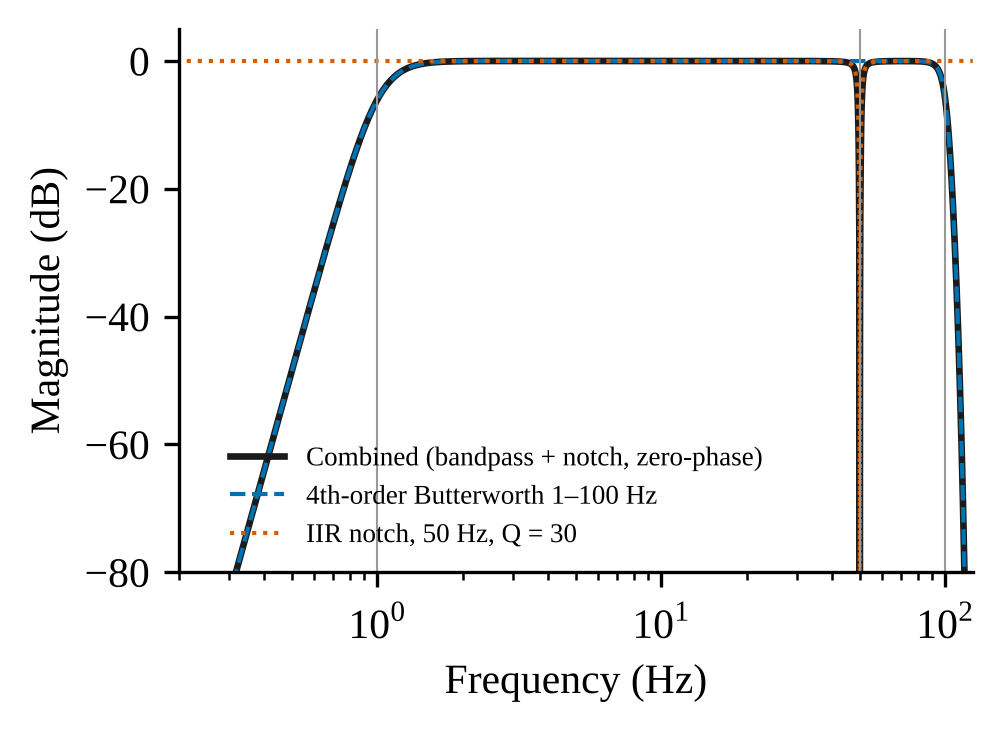
\includegraphics[width=\columnwidth]{figs/fig_filter_col.png}
\caption{Magnitude response of the conditioning filters in the effective forward--backward form.}
\label{fig:filter}
\end{figure}

\begin{table}[!t]
\caption{Detected P100 latency in ms (mean $\pm$ SD over 50 trials per class).}
\label{tab:p100}
\centering\footnotesize
\begin{tabular}{@{}lcccc@{}}
\toprule
Class & True & Raw & Zero-phase & Single-pass\\
\midrule
Healthy Control & 100 & $101.8\pm2.3$ & $100.6\pm1.9$ & $101.1\pm1.8$ \\
Glaucoma & 108 & $107.4\pm2.7$ & $108.0\pm2.9$ & $108.2\pm2.3$ \\
Optic Neuritis/CVI & 140 & $141.3\pm2.5$ & $140.8\pm2.1$ & $141.0\pm2.7$
\\
\bottomrule
\end{tabular}
\end{table}

Table~\ref{tab:p100} gives the detected P100 latencies. With zero-phase conditioning, \nWithin{} of \nTrials{} trials (99.3\%) were within one sample period (4~ms) of the ground truth, and the largest error was 8~ms, in one Glaucoma trial; the class means differ from the truth by $+0.64$, $0.00$ and $+0.80$~ms. The single-pass implementation, whose group delay is \gdTen{}, \gdTwenty{} and \gdThirty{}~ms at 10, 20 and 30~Hz, gave class means within 0.5~ms of the zero-phase means (Fig.~\ref{fig:p100}); this difference is below one sample.

\begin{figure}[!t]
\centering
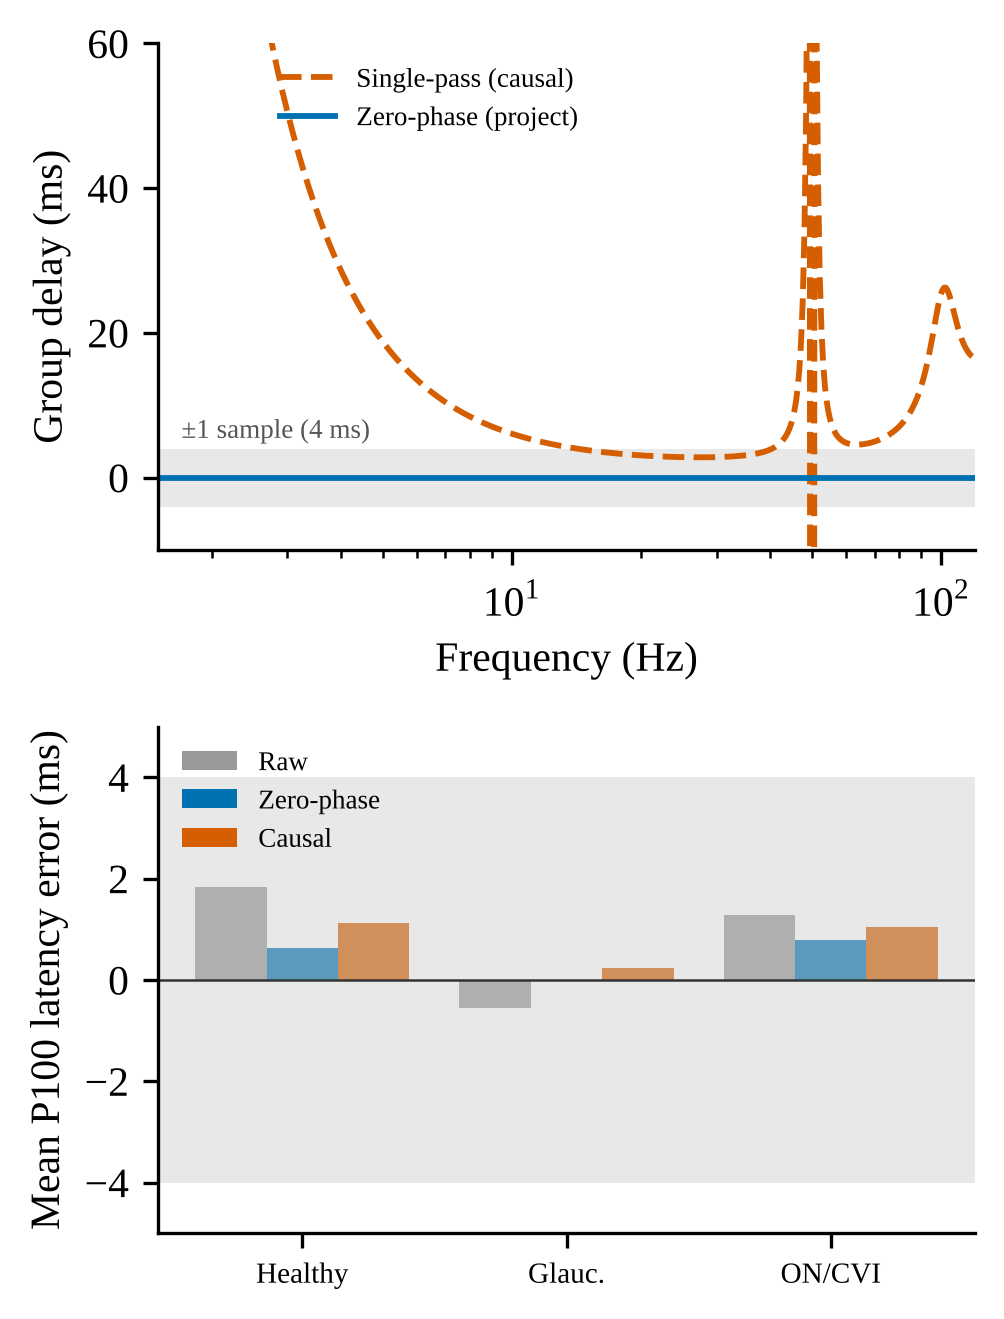
\includegraphics[width=\columnwidth]{figs/fig_p100_col.png}
\caption{Top: group delay of the single-pass filters versus the zero-phase pipeline (shaded band: $\pm1$ sample, 4~ms). Bottom: mean P100 latency error by class (shaded band: $\pm4$~ms).}
\label{fig:p100}
\end{figure}

\subsection{Synthetic MRI and the foreground mask}
The generators behave as specified: the mean intensity of the atrophy block in the Glaucoma volume is \atrophyROI{} against about 100 elsewhere, and that of the lesion block in the Optic Neuritis/CVI volume is \lesionROI{}. The 60th-percentile mask zeroes exactly 60\% of the voxels of every volume. In the Glaucoma volume it removes the whole atrophy block (\retAtrophy\% retained), while \retLesion\% of the lesion block is retained in the Optic Neuritis/CVI volume.

\subsection{Model size and cost}
CAFN has \nParams{} trainable parameters and about \nMACsG{} billion MACs per sample (Table~\ref{tab:params}). The spatial encoder holds \pSpatial\% of the parameters, the fusion module \pFusion\%, the temporal encoder \pTemporal\%. The compute is concentrated in the early 3D stages: the first residual block alone accounts for \pBlockOne\% of the MACs and the first two for \pBlocksOneTwo\%, whereas the fusion module accounts for well under 1\%.

\begin{table}[!t]
\caption{Trainable parameters and MACs (millions) per sample at the default configuration.}
\label{tab:params}
\centering\footnotesize
\begin{tabular}{@{}lrr@{}}
\toprule
Component & Parameters & MACs (M)\\
\midrule
Spatial encoder (3D residual CNN) & 883,472 & 2,520.78 \\
Temporal encoder (1D CNN) & 37,968 & 3.52 \\
Cross-attention fusion (attention, FFN, LN) & 132,480 & 7.08 \\
Classification heads (3) & 1,161 & 0.00 \\
\midrule
Total & 1,055,081 & 2,531.38
\\
\bottomrule
\end{tabular}
\end{table}

\subsection{Software verification}
The repository contains 86 test functions in 12 files (78 unit and 8 integration tests). Statement coverage reconstructed from the recorded coverage data is \nHit{} of \nStmts{} statements (\covTotal\%), with \nFullMods{} of \nMods{} modules fully covered; the lowest is the training script (\covTrain\%), whose uncovered statements are mainly the command-line entry point. The tests assert shapes, value ranges, normalisation of attention rows, determinism, input validation and end-to-end gradient flow.

\subsection{Training acceptance criteria}
The training-loop integration tests use a scaled-down model ($d_{\mathrm{model}}=32$, 2 heads, 8+8 tokens, $32^3$ MRI, 200-sample VEP). The loss and accuracy criteria of Table~\ref{tab:accept} are tested on 24 synthetic samples over 15 epochs, the other two on 8 samples over 2 epochs. The tests assert thresholds, not point values, so the exact loss and accuracy reached are not part of the recorded results.

\begin{table}[!t]
\caption{Training acceptance criteria asserted by the integration tests.}
\label{tab:accept}
\centering\footnotesize
\begin{tabular}{@{}p{0.2\columnwidth}p{0.7\columnwidth}@{}}
\toprule
Criterion & Specification\\
\midrule
Loss & Final training loss $<0.7\times$ initial training loss\\
Accuracy & Validation accuracy of the fused head $>0.5$ (chance: 0.33)\\
No validation set & Training runs; validation-loss history is empty\\
Checkpoint & Saved and reloaded model reproduces the fused logits exactly\\
\bottomrule
\end{tabular}
\end{table}

\section{Discussion}\label{sec:discussion}
\subsection{Interpretation}
The conditioning results confirm the intended behaviour: the pass-band is flat, the 50~Hz component is removed by about \notchDb~dB in the ideal response, and P100 latency is recovered to within one sample on average, preserving the ordering of the classes. The measured \nMainsDb~dB mains reduction is much smaller than the ideal response, but this is a noise-floor effect: after filtering, the fitted 50~Hz amplitude is of the same order as the amplitude fitted at 47~Hz, so the figure is a lower bound on the notch's attenuation. The benefit of zero-phase over single-pass filtering could not be demonstrated on these data: the smooth, low-frequency synthetic P100 is insensitive to a delay of a few milliseconds. The case for zero-phase processing therefore rests on the principle that latency is the clinical quantity \cite{odom2016}, not on an empirical gain at 250~Hz.

\subsection{Design observations}
The mask result shows that the placeholder preprocessing is not neutral: by construction it zeroes 60\% of every volume and, in the Glaucoma volume, removes the atrophy block entirely. Conclusions about what the spatial encoder can learn from synthetic MRI thus depend on the preprocessing and do not transfer to skull-stripped real scans. With 16 temporal tokens over 2~s, the P100 peaks of Healthy Control (100~ms) and Glaucoma (108~ms) fall in the same nominal 125~ms token, so the tokens must not be read as calibrated time bins and the attention heatmap does not point to a millisecond. The computational profile suggests that any reduction in training time should target the early 3D stages, not the fusion module.

\subsection{Explainability and comparison}
The design follows intermediate fusion of learned features \cite{baltrusaitis2019,ramachandram2017} and uses cross-attention in the sense of \cite{tsai2019,lu2019}, with queries from the structural stream and keys and values from the electrophysiological stream. It differs from those works in modality, in scale (about one million parameters) and, most importantly, in evidence: they report benchmark results, whereas this paper reports engineering verification on synthetic data, so no numerical comparison with published classification results is attempted. Because attention weights and saliency maps are not automatically faithful \cite{jain2019,wiegreffe2019,adebayo2018}, the outputs are inspection aids whose faithfulness remains to be tested.

\subsection{Limitations}
(i)~All learning experiments use synthetic data that are deliberately simple; no statement about diagnostic accuracy, sensitivity or generalisation is possible. (ii)~Training was not executed for this paper, so no measured curves are reported. (iii)~Complexity figures are analytic, not profiled, and coverage was reconstructed from recorded data. (iv)~The foreground mask is a placeholder. (v)~No unimodal or concatenation baseline and no ablation of the auxiliary heads exists, so the added value of cross-attention is untested. (vi)~Tokens are learned, uncalibrated feature positions.

\section{Conclusion and Future Work}\label{sec:conclusion}
This paper described and verified CAFN, a cross-attention fusion network for paired 3D structural MRI and VEP. The two modalities are brought to a common token space through one configuration-driven pipeline, fused by letting 64 spatial tokens query 16 temporal tokens, and supervised by a fused head and two auxiliary heads. On synthetic data, zero-phase conditioning recovered P100 latency within one sample in \nWithin{} of \nTrials{} records, the model needs \nParams{} parameters, and an 86-test suite covers \covTotal\% of statements. No diagnostic claim is made. The next step is data, not architecture: with a labelled, paired cohort, the priorities are (1)~training with patient-level splits and reporting of sensitivity, specificity, AUC and calibration; (2)~unimodal and concatenation baselines and ablations of the auxiliary loss and token counts; (3)~validated skull-stripping in place of the percentile mask; (4)~sanity checks of Grad-CAM and attention against clinician-marked regions; and (5)~anatomically grounded tokens aligned with the VEP landmarks N75, P100 and N135.

\section*{Acknowledgment}
The author thanks \todo{guide name and designation} for guidance throughout this project.

\begin{thebibliography}{39}
\bibitem{tham2014}
Y.-C. Tham, X. Li, T. Y. Wong, H. A. Quigley, T. Aung, and C.-Y. Cheng, ``Global prevalence of glaucoma and projections of glaucoma burden through 2040: A systematic review and meta-analysis,'' \emph{Ophthalmology}, vol. 121, no. 11, pp. 2081--2090, 2014, doi: 10.1016/j.ophtha.2014.05.013.
\bibitem{gupta2006}
N. Gupta, L.-C. Ang, L. No\"{e}l de Tilly, L. Bidaisee, and Y. H. Y\"{u}cel, ``Human glaucoma and neural degeneration in intracranial optic nerve, lateral geniculate nucleus, and visual cortex,'' \emph{Brit. J. Ophthalmol.}, vol. 90, no. 6, pp. 674--678, 2006, doi: 10.1136/bjo.2005.086769.
\bibitem{halliday1972}
A. M. Halliday, W. I. McDonald, and J. Mushin, ``Delayed visual evoked response in optic neuritis,'' \emph{Lancet}, vol. 299, no. 7758, pp. 982--985, 1972, doi: 10.1016/S0140-6736(72)91155-5.
\bibitem{sakki2018}
H. E. A. Sakki, N. J. Dale, J. Sargent, T. Perez-Roche, and R. Bowman, ``Is there consensus in defining childhood cerebral visual impairment? A systematic review of terminology and definitions,'' \emph{Brit. J. Ophthalmol.}, vol. 102, no. 4, pp. 424--432, 2018, doi: 10.1136/bjophthalmol-2017-310694.
\bibitem{odom2016}
J. V. Odom \emph{et al.}, ``ISCEV standard for clinical visual evoked potentials: (2016 update),'' \emph{Documenta Ophthalmol.}, vol. 133, no. 1, pp. 1--9, 2016, doi: 10.1007/s10633-016-9553-y.
\bibitem{calhoun2016}
V. D. Calhoun and J. Sui, ``Multimodal fusion of brain imaging data: A key to finding the missing link(s) in complex mental illness,'' \emph{Biol. Psychiatry, Cogn. Neurosci. Neuroimaging}, vol. 1, no. 3, pp. 230--244, 2016, doi: 10.1016/j.bpsc.2015.12.005.
\bibitem{kamnitsas2017}
K. Kamnitsas \emph{et al.}, ``Efficient multi-scale 3D CNN with fully connected CRF for accurate brain lesion segmentation,'' \emph{Med. Image Anal.}, vol. 36, pp. 61--78, 2017, doi: 10.1016/j.media.2016.10.004.
\bibitem{cicek2016}
\"{O}. \c{C}i\c{c}ek, A. Abdulkadir, S. S. Lienkamp, T. Brox, and O. Ronneberger, ``3D U-Net: Learning dense volumetric segmentation from sparse annotation,'' in \emph{Proc. Med. Image Comput. Comput.-Assist. Intervent. (MICCAI)}, 2016, pp. 424--432, doi: 10.1007/978-3-319-46723-8\_49.
\bibitem{he2016}
K. He, X. Zhang, S. Ren, and J. Sun, ``Deep residual learning for image recognition,'' in \emph{Proc. IEEE Conf. Comput. Vis. Pattern Recognit. (CVPR)}, 2016, pp. 770--778, doi: 10.1109/CVPR.2016.90.
\bibitem{isensee2019}
F. Isensee \emph{et al.}, ``Automated brain extraction of multisequence MRI using artificial neural networks,'' \emph{Hum. Brain Mapp.}, vol. 40, no. 17, pp. 4952--4964, 2019, doi: 10.1002/hbm.24750.
\bibitem{hoopes2022}
A. Hoopes, J. S. Mora, A. V. Dalca, B. Fischl, and M. Hoffmann, ``SynthStrip: Skull-stripping for any brain image,'' \emph{NeuroImage}, vol. 260, Art. no. 119474, 2022, doi: 10.1016/j.neuroimage.2022.119474.
\bibitem{cardoso2022}
M. J. Cardoso \emph{et al.}, ``MONAI: An open-source framework for deep learning in healthcare,'' 2022, \emph{arXiv:2211.02701}.
\bibitem{butterworth1930}
S. Butterworth, ``On the theory of filter amplifiers,'' \emph{Exp. Wireless Wireless Eng.}, vol. 7, pp. 536--541, 1930.
\bibitem{gustafsson1996}
F. Gustafsson, ``Determining the initial states in forward-backward filtering,'' \emph{IEEE Trans. Signal Process.}, vol. 44, no. 4, pp. 988--992, 1996, doi: 10.1109/78.492552.
\bibitem{oppenheim2010}
A. V. Oppenheim and R. W. Schafer, \emph{Discrete-Time Signal Processing}, 3rd ed. Upper Saddle River, NJ, USA: Pearson, 2010.
\bibitem{baltrusaitis2019}
T. Baltru\v{s}aitis, C. Ahuja, and L.-P. Morency, ``Multimodal machine learning: A survey and taxonomy,'' \emph{IEEE Trans. Pattern Anal. Mach. Intell.}, vol. 41, no. 2, pp. 423--443, 2019, doi: 10.1109/TPAMI.2018.2798607.
\bibitem{ramachandram2017}
D. Ramachandram and G. W. Taylor, ``Deep multimodal learning: A survey on recent advances and trends,'' \emph{IEEE Signal Process. Mag.}, vol. 34, no. 6, pp. 96--108, 2017, doi: 10.1109/MSP.2017.2738401.
\bibitem{vaswani2017}
A. Vaswani \emph{et al.}, ``Attention is all you need,'' in \emph{Proc. Adv. Neural Inf. Process. Syst. (NeurIPS)}, vol. 30, 2017, pp. 5998--6008.
\bibitem{dosovitskiy2021}
A. Dosovitskiy \emph{et al.}, ``An image is worth 16\texttimes16 words: Transformers for image recognition at scale,'' in \emph{Proc. Int. Conf. Learn. Represent. (ICLR)}, 2021.
\bibitem{tsai2019}
Y.-H. H. Tsai, S. Bai, P. P. Liang, J. Z. Kolter, L.-P. Morency, and R. Salakhutdinov, ``Multimodal transformer for unaligned multimodal language sequences,'' in \emph{Proc. 57th Annu. Meeting Assoc. Comput. Linguistics}, 2019, pp. 6558--6569, doi: 10.18653/v1/P19-1656.
\bibitem{lu2019}
J. Lu, D. Batra, D. Parikh, and S. Lee, ``ViLBERT: Pretraining task-agnostic visiolinguistic representations for vision-and-language tasks,'' in \emph{Proc. Adv. Neural Inf. Process. Syst. (NeurIPS)}, vol. 32, 2019, pp. 13--23.
\bibitem{selvaraju2017}
R. R. Selvaraju, M. Cogswell, A. Das, R. Vedantam, D. Parikh, and D. Batra, ``Grad-CAM: Visual explanations from deep networks via gradient-based localization,'' in \emph{Proc. IEEE Int. Conf. Comput. Vis. (ICCV)}, 2017, pp. 618--626, doi: 10.1109/ICCV.2017.74.
\bibitem{jain2019}
S. Jain and B. C. Wallace, ``Attention is not explanation,'' in \emph{Proc. Conf. North Amer. Chapter Assoc. Comput. Linguistics: Human Lang. Technol. (NAACL-HLT)}, 2019, pp. 3543--3556, doi: 10.18653/v1/N19-1357.
\bibitem{wiegreffe2019}
S. Wiegreffe and Y. Pinter, ``Attention is not not explanation,'' in \emph{Proc. Conf. Empirical Methods Natural Lang. Process. 9th Int. Joint Conf. Natural Lang. Process. (EMNLP-IJCNLP)}, 2019, pp. 11--20, doi: 10.18653/v1/D19-1002.
\bibitem{adebayo2018}
J. Adebayo, J. Gilmer, M. Muelly, I. Goodfellow, M. Hardt, and B. Kim, ``Sanity checks for saliency maps,'' in \emph{Proc. Adv. Neural Inf. Process. Syst. (NeurIPS)}, vol. 31, 2018, pp. 9505--9515.
\bibitem{vanessen2013}
D. C. Van Essen, S. M. Smith, D. M. Barch, T. E. J. Behrens, E. Yacoub, and K. Ugurbil, ``The WU-Minn Human Connectome Project: An overview,'' \emph{NeuroImage}, vol. 80, pp. 62--79, 2013, doi: 10.1016/j.neuroimage.2013.05.041.
\bibitem{benson2018}
N. C. Benson \emph{et al.}, ``The Human Connectome Project 7 Tesla retinotopy dataset: Description and population receptive field analysis,'' \emph{J. Vis.}, vol. 18, no. 13, Art. no. 23, 2018, doi: 10.1167/18.13.23.
\bibitem{lamontagne2019}
P. J. LaMontagne \emph{et al.}, ``OASIS-3: Longitudinal neuroimaging, clinical, and cognitive dataset for normal aging and Alzheimer disease,'' \emph{medRxiv}, 2019, doi: 10.1101/2019.12.13.19014902.
\bibitem{gramfort2013}
A. Gramfort \emph{et al.}, ``MEG and EEG data analysis with MNE-Python,'' \emph{Front. Neurosci.}, vol. 7, Art. no. 267, 2013, doi: 10.3389/fnins.2013.00267.
\bibitem{goldberger2000}
A. L. Goldberger \emph{et al.}, ``PhysioBank, PhysioToolkit, and PhysioNet: Components of a new research resource for complex physiologic signals,'' \emph{Circulation}, vol. 101, no. 23, pp. e215--e220, 2000, doi: 10.1161/01.CIR.101.23.e215.
\bibitem{paszke2019}
A. Paszke \emph{et al.}, ``PyTorch: An imperative style, high-performance deep learning library,'' in \emph{Proc. Adv. Neural Inf. Process. Syst. (NeurIPS)}, vol. 32, 2019, pp. 8024--8035.
\bibitem{virtanen2020}
P. Virtanen \emph{et al.}, ``SciPy 1.0: Fundamental algorithms for scientific computing in Python,'' \emph{Nature Methods}, vol. 17, no. 3, pp. 261--272, 2020, doi: 10.1038/s41592-019-0686-2.
\bibitem{harris2020}
C. R. Harris \emph{et al.}, ``Array programming with NumPy,'' \emph{Nature}, vol. 585, no. 7825, pp. 357--362, 2020, doi: 10.1038/s41586-020-2649-2.
\bibitem{hunter2007}
J. D. Hunter, ``Matplotlib: A 2D graphics environment,'' \emph{Comput. Sci. Eng.}, vol. 9, no. 3, pp. 90--95, 2007, doi: 10.1109/MCSE.2007.55.
\bibitem{zhou2024camf}
Z. Zhou, A. Orlichenko, G. Qu, Z. Fu, V. D. Calhoun, Z. Ding, and Y.-P. Wang, ``An interpretable cross-attentive multi-modal MRI fusion framework for schizophrenia diagnosis,'' 2024, \emph{arXiv:2404.00144}.
\bibitem{dhar2025drifa}
J. Dhar, N. Zaidi, M. Haghighat, S. Roy, P. Goyal, A. Alavi, and V. Kumar, ``Multimodal fusion learning with dual attention for medical imaging,'' in \emph{Proc. IEEE/CVF Winter Conf. Appl. Comput. Vis. (WACV)}, 2025, pp. 4362--4371, doi: 10.1109/WACV61041.2025.00428.
\bibitem{hu2018}
J. Hu, L. Shen, and G. Sun, ``Squeeze-and-excitation networks,'' in \emph{Proc. IEEE Conf. Comput. Vis. Pattern Recognit. (CVPR)}, 2018, pp. 7132--7141, doi: 10.1109/CVPR.2018.00745.
\bibitem{liuzzi2022ds003568}
L. Liuzzi, K. Chang, H. Keren, C. Zheng, D. Saha, D. Nielson, and A. Stringaris, ``Mood induction in MDD and healthy adolescents,'' OpenNeuro dataset ds003568, v1.0.4, 2023, doi: 10.18112/openneuro.ds003568.v1.0.4 (see also L. Liuzzi \emph{et al.}, ``Electrophysiological correlates of mood and reward dynamics in human adolescents,'' \emph{bioRxiv}, 2021, doi: 10.1101/2021.03.04.433969).
\bibitem{ds007181}
L. Li, Q. Han, H. Bai, X. Zhang, Y. Liu, and C. He, ``Structural MRI, resting-state fMRI, and PSG/EEG dataset of zoster-associated neuralgia,'' OpenNeuro dataset ds007181, v1.0.1, 2026, doi: 10.18112/openneuro.ds007181.v1.0.1.
\end{thebibliography}


\begin{biography}{}{Mishthi Jain}
is a B.Tech.\ student in Computer Science and Engineering (Artificial Intelligence and Machine Learning) at the Vellore Institute of Technology, Chennai, India. \todo{short biography and research interests}
\end{biography}
\EOD
\end{document}
